\section{Device Driver}

\subsection{Lerninhalt}

\begin{itemize}
   \item Sie kennen die Klassifizierung von \emph{Device Driver}
   \item Sie kennen eine Art, wie ein Dateityp bestimmt werden kann
   \item Sie kennen die Major- und Minornummer
   \item Sie kennen die \emph{Char Device Drivers}
   \item Sie kennen die \emph{Block Device Drivers}
   \item Sie kennen die \emph{Network Device Drivers}
\end{itemize}

\subsection{Device Driver}

Unter Linux werden Geräte als Dateien repräresentiert. Natürlich sind dies keine normalen Dateien, sondern \emph{virtuelle Dateien} (Kaptiel \ref{sec:vfs}).
Die Gerätedateien in einem laufenden Linux-System sind unter dem Verzeichnis \emph{/dev} abgebildet. Die Tabelle \ref{tab:dev_tab} beschreibt einige der Gerätedateien,
die dort zu finden sind.

\begin{longtable}{| l | l | p{10cm} |} \hline
   \textbf{Gerätedatei} & \textbf{Typ} & \textbf{Beschreibung} \\ \hline
   /dev/sdXY         & Block & Bezeichnet ursprünglich nur SCSI Datenträger\footnote{Heutzutage werden alle Datenträger, die
                               über das SCSI-Framework angebunden sind, so bezeichnet. Da SATA dieselben Befehle wie SCSI benützt
                               und auch USB-Datenträger SCSI-Befehle über das USB-Protokoll übertragen, werden diese Treiber mit
                               dem SCSI-Framework implementiert.}. Das X steht für die alphabetische Nummerierung
                               der Datenträger und das Y steht für die Partitionsnummer, falls vorhanden. So steht \emph{/dev/sda} 
                               für den ersten Datenträger und \emph{/dev/sda2} für die zweite Partition auf dem ersten Datenträger. \\ \hline
   /dev/input/mouseX & Char & Pro angeschlossene Maus wird eine solche Datei erzeugt. Darin steht, welche Tasten gedrückt sind und die aktuelle Positionsverschiebung. \\ \hline
   /dev/input/mice   & Char & Kombiniert alle Inhalte der mouseX-Dateien in einer Datei. \\ \hline
   /dev/zero         & Char & Gibt immer 0 aus (virtuelles Device).\\ \hline
   /dev/random       & Char & Gibt pseudo Zufallszahlen aus (virtuelles Device).\\ \hline
   /dev/urandom      & Char & Gibt echte Zufallszahlen aus (virtuelles Device).\\ \hline
   /dev/mem          & Char & Entspricht dem physikalischen Arbeitsspeicher. \\ \hline
   \caption{Gerätedateien unter \emph{/dev}}
   \label{tab:dev_tab}
\end{longtable}

Um ein Geräte anzusteuern, werden Dateioperationen (Kapitel \ref{sec:syscall} - \emph{\nameref{sec:syscall}}) auf die Gerätedatei ausgeführt. Wie das funktioniert, wird in diesem Kaptiel genauer
beschrieben.

\subsection{Klassifizierung}

Unter Linux gibt es drei Arten von \keyword{Device Driver}, die \keyword{Char Device Driver}, die \keyword{Block Device Driver} und die \keyword{Network Device Driver}. Sie unterscheiden sich in 
der Weise, wie auf diese Geräte zugegriffen werden kann.
\clearpage
\begin{description}[leftmargin=5cm]
   \item[Char Device Driver]
         Character (Char) Device Driver sind die einfachsten und zugleich die meist verwendeten Treiberarten. Diese Gerätedateien verhalten sich wie ein \keyword{Stream}. Die Geräte werden byteweise
         geschrieben und/oder gelesen. Beispiele für  Dateioperationen: \emph{open()}, \emph{read()}, \emph{write()}, \emph{flush()} und \emph{release()}. \\

         Beispiele:
         \begin{itemize}
            \item Eingabegeräte (Maus, Keyboard, Joystick)
            \item Aufnahmegeräte (Kamera, Mikrophone)
            \item Ausgabegeräte (Kopfhörer, Lautsprecher)
            \item Sensoren (Temparatur, Druck, Luftfeuchtigkeit)
         \end{itemize}

   \item[Block Device Driver]
         Auf block-orientierte Geräte kann nicht byteweise zugegriffen werden. Es werden immer ganze Blöcke (meist 512-Bytes) gelesen oder geschrieben. Der Gerätedatei liegt ein Filesystem (z.B. ext4) zugrunde,
         das zuerst über \emph{mount} verbunden werden muss. Der Kernel führt für diese Treiberart einen \keyword{I/O-Cache} und \keyword{I/O-Scheduler}, um die Geschwindigkeit des Systems zu erhöhen. Implementierte
         Beispiele für Dateioperationen:  \emph{open()}, \emph{media\_changed()}, \emph{release()}. Auf die Datei geschrieben bzw. gelesen wird nicht über die normale Dateioperation, sondern über ein anderes Interface. \\

         Beispiele:
         \begin{itemize}
            \item Feste Datenträger (SCSI-, SATA-, IDE-Datenträger)
            \item Wechseldatenträger (USB-Stick/Festplatte, CD-ROM, DVD)
         \end{itemize}

   \item[Network Device Driver]
         Netzwerk-Treiber sind weder byte- noch blockweise zugreifbar, sie sind Packet-orientiert und aus diesem Grund nicht im Verzeichnis \emph{/dev} zu finden. Anstelle von Gerätedateien werden bei diesen Treibern 
         sogenannte \keyword[Interfaces]{Interfaces} erzeugt. Die Interfaces können über den Befehl \emph{ifconfig -a} angezeigt werden. Um die Interfaces zu nutzen, muss zuerst eine Verbindung aufgebaut werden. Beispiele für 
         die Operation des Interfaces sind: \emph{open()}, \emph{stop()}, \emph{set\_config()}, \emph{hard\_start\_xmit()}, \emph{get\_stat()} und \emph{tx\_timeout()}. \\

         Beispiele:
         \begin{itemize}
            \item Kabelgebundene Netzwerke (Ethernet, USB)
            \item Kabellose Netzwerke (WLAN, Bluetooth)
         \end{itemize}
         
\end{description} \hfill

Über \emph{ls -l} kann bestimmt werden, ob eine Datei eine Gerätedatei ist und von welchem Typ sie ist. Die Abbildung \ref{fig:file_type} zeigt, wie das geht.
\clearpage
\begin{figure}[h!]
   \begin{center}
      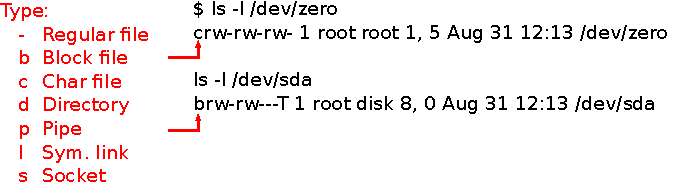
\includegraphics{images/file_type}
   \end{center}
   \caption{Bestimmung des Dateityps}
   \label{fig:file_type}
\end{figure}

\subsection{Major- und Minornummer}

Der Linux-Kernel verwendet zur Identifikation von Treibern sogenannte Major- und Minornummern. Jeder Char- und Block-Gerätetreiber muss eine Majornummer beim Kernel registieren.
Beim Erstellen von Gerätedateien werden diese über die Majornummer mit dem Treiber verbunden. \\

Die Datei \emph{/proc/devices} beinhaltet alle registrierten Majornummer und den dazugehörigen Treiber (Listing \ref{proc_devices}).
\begin{lstlisting}[label=proc_devices,caption=/proc/devices]
Character devices:
  1 mem
  4 /dev/vc/0
  4 tty
  4 ttyS
  5 /dev/tty
  5 /dev/console
..

Block devices:
259 blkext
  7 loop
  8 sd
 11 sr
..
\end{lstlisting} \hfill

Um eine Gerätedatei mit dem Treiber \emph{mem} zu erstellen, kann mit dem Befehl \emph{mknod} erstellet werden (Listing \ref{mknod}).
Dabei ist \emph{zero} der Dateiname, \emph{c} besagt, dass es eine Char-Datei sein soll und \emph{1} bzw. \emph{5} stehen für die Major- und Minornummer.
Die Datei verhält sich anschliessend gleich wie \emph{/dev/zero}. Das liegt daran, dass beide Dateien mit den gleichen Major- und Minornummer erstell wurden.
\begin{lstlisting}[label=mknod,caption=mknod]
$ sudo mknod zero c 1 5

$ ls -l /dev/zero zero
<@\textcolor{red}{c}@>rw-rw-rw- 1 root root <@\textcolor{red}{1, 5}@> Aug 31 12:13 /dev/zero
<@\textcolor{red}{c}@>rw-r--r-- 1 root root <@\textcolor{red}{1, 5}@> Aug 31 17:40 zero
\end{lstlisting} \hfill

Die Minornummer ist abhängig von der Implementation des Treibers. Der Treiber \emph{mem} verwendet die Minornummer um \emph{/dev/null}, \emph{/dev/zero}, etc. zu unterscheiden.
Der SCSI-Treiber unterscheidet damit die Partitionen.

\subsection{Char Device Driver}

Zuerst wird der \emph{Char Device Driver} besprochen. Anhand eines einfachen Tastaturtreibers soll dies genauer erklärt werden. Ein Tastaturtreiber erstellt an geeigneter
Stelle unter \emph{/dev} eine neue Gerätedatei (z.B. \emph{/dev/keyboard}). Ein Userspace-Programm wird dann die Datei öffnen und die Tastaturevents auslesen. Ist das 
Programm fertig, so wird die Datei geschlossen. \\

Der Treiber bietet sogenannte \keyword{Dateioperationen} an. Dadurch wird der Treiber über Funktionsaufrufe wie \emph{open()}, \emph{read()} und \emph{close()} informiert
und kann darauf reagieren. Im Falle eines USB-Tastaturtreibers würde bei einem Leseaufruf das Gerät nach neuen Events abgefragt. Falls neue Events vorhanden sind, werden diese dem Userspace-Programm
zurückgeliefert.

\subsubsection{Initialisierung des Char-Treibers}

Als erstes sollte eine Majornummer reserviert werden, um diesen Treiber eindeutig zu indentifizieren. Das geschieht mit der Funktion \emph{alloc\_chrdev\_region()}.
\begin{lstlisting}[caption=Majornummer registrieren für Char-Treiber]
int alloc_chrdev_region(dev_t *dev, unsigned int firstminor, unsigned int count, char *name);
\end{lstlisting}
In die Struktur \emph{dev\_t} wird die freie Majornummer vom Kernel geschrieben. \emph{firstminor} gibt an, welche die erste Minorzahl
sein soll. \emph{Count} gibt die Gesamtanzahl an. Für die meisten Treiber haben Minornummern keine besondere Bedeutung
und somit wird nur eine Minornummer erstellt. \emph{name} ist der Treibername und erscheint unter \emph{/proc/devices}. \\

Danach kann die zentrale Struktur \emph{cdev} für den Char-Treiber erstellt werden. Die Funktion \emph{cdev\_alloc()} alloziert und
\emph{cdev\_init()} initialisiert den Speicher. Zum Schluss muss der neue Treiber über \emph{cdev\_add()} dem Kernel bekannt gemacht
werden.
\begin{lstlisting}[caption=Funktion für den Char-Treiber]
struct cdev *cdev_alloc(void);
void cdev_init(struct cdev *dev, struct file_operations *fops);
int cdev_add(struct cdev *dev, dev_t num, unsigned int count);
\end{lstlisting}
Interessant ist, dass bei \emph{cdev\_init()} eine Struktur names \emph{file\_operations} mitgegeben wird. Darin kann das Verhalten der Dateioperationen
definiert werden.

\subsubsection{Dateioperationen des Char-Treibers}

Die vollständige \emph{file\_operation} Struktur ist unter \emph{include/linux/fs.h} zu finden. Das Listing \ref{lst:char_fileop} zeigt nur einen Ausschnitt. 
Um den Char-Treiber zu benutzen, müssen nur noch die gewünschten Funktionen implementiert werden.

\begin{lstlisting}[label=lst:char_fileop,caption=Dateioperationen]
struct file_operations {
   struct module *owner;
   ssize_t (*read) (struct file *, char __user *, size_t, loff_t *);
   ssize_t (*write) (struct file *, const char __user *, size_t, loff_t *);
   ssize_t (*read_iter) (struct kiocb *, struct iov_iter *);
   ssize_t (*write_iter) (struct kiocb *, struct iov_iter *);
   int (*open) (struct inode *, struct file *);
   int (*flush) (struct file *, fl_owner_t id);
   int (*release) (struct inode *, struct file *);
   ..
};
\end{lstlisting}

\subsubsection{Read-Dateioperation}

Für das Beispiel mit der Tastatur muss nur die Read-Methode implementiert werden. Anstatt eine Anbindung an ein physikalisches
Gerät zu programmieren, wird hier einfach immer der Buchstabe \emph{a} ausgegeben.


\begin{lstlisting}
static ssize_t keyboard_read(struct file *file, char __user *buf, size_t buf_size, loff_t *offset)
{
        // write 'a' into buffer
        copy_to_user(buf, "a", 1);

        // one byte read
        return 1;
}
\end{lstlisting}

\subsubsection{Komplettes Char Driver-Beispiel}

Das vollständige Beispiel ist in Listing \ref{lst:char_driver} abgebildet.

\begin{lstlisting}[label=lst:char_driver,caption=Char Driver]
#include <linux/version.h>
#include <linux/kernel.h>
#include <linux/init.h>
#include <linux/module.h>
#include <linux/types.h>
#include <linux/kdev_t.h>
#include <linux/fs.h>
#include <linux/device.h>
#include <linux/cdev.h>
#include <linux/uaccess.h>

static dev_t dev_no; // major number
static struct cdev dev; // char device driver structure

static ssize_t keyboard_read(struct file *f, char __user *buf, size_t len, loff_t *off)
{
        // write 'a' into buffer
        copy_to_user(buf, "a", 1);

        // one byte read
        return 1;
}

static struct file_operations keyboard_fops =
{
        .owner = THIS_MODULE,
        .read = keyboard_read,
};

static int __init keyboard_init (void)
{
        // register major number
        if (alloc_chrdev_region(&dev_no, 0, 1, "keyboard") < 0) {
                return -1;
        }

        // init char device driver
        cdev_init(&dev, &keyboard_fops);
        if (cdev_add(&dev, dev_no, 1) == -1) {
                unregister_chrdev_region(dev_no, 1);
                return -1;
        }

        return 0;
}

static void __exit keyboard_release (void)
{
        // release char driver structure
        cdev_del(&dev);

        // release major number
        unregister_chrdev_region(dev_no, 1);
}

module_init(keyboard_init);
module_exit(keyboard_release);
\end{lstlisting}

\subsubsection{Verwendung von Charactergeräten}

Um den Treiber zu testen, muss er nur noch kompiliert und installiert werden:
\begin{lstlisting}
$ make
$ sudo insmod mykeyboard
\end{lstlisting} \hfill

Um die zugewiesene Majornummer herauszufinen, kann in der Datei \emph{/proc/devices} nachgeschaut werden. Danach
wird die Gerätedatei mit dieser Nummer erstellt.
\begin{lstlisting}
$ grep keyboard /proc/devices
251 keyboard

$ sudo mknod /dev/keyboard c 251 0
\end{lstlisting}

Nun kann die Gerätedatei ausgelesen werden:
\begin{lstlisting}
$ head /dev/keyboard 
a
a
a
a
a
a
a
a
a
a
\end{lstlisting}

\subsection{Block Device Driver}

Der \emph{Block Device Driver} ist in vielerlei Hinsicht ähnlich zum \emph{Char Device Driver}. Das Konzept der Major- und Minornummer existiert hier ebenfalls und 
auch die Dateioperationen gibt es. Nur werden beim \emph{Block Device Driver} die Daten anders gelesen und geschrieben. Das ergibt vorallem deshalb Sinn, weil hierbei
grössere Dateimengen übertragen werden, die durch \keyword[Cache]{Caching} und \keyword{Scheduling} effizient gestaltet werden sollen.

\subsubsection{Registrierung der Majornummer für Block-Treiber}

Auch hier soll als erstes die Majornummer reserviert werden. Wenn man die Datei \emph{/proc/devices} ansieht, merkt man, dass die Nummerierung von Char- und Block-Devices
unterschiedlich ist. Deshalb muss auch die Majornummer für Blockgeräte anders reserviert werden (Listing \ref{register_blkdev}).

\begin{lstlisting}[label=register_blkdev,caption=Majornummer registrieren für Block-Treiber]
int register_blkdev(unsigned int major, const char *name);
int unregister_blkdev(unsigned int major, const char *name);
\end{lstlisting}

Falls die Majornummer nicht fest bestimmt werden soll, kann für \emph{major} einfach \emph{0} übergeben werden. Dadurch wird automatisch eine freie Nummer als Return-Wert zugewiesen. \\

\subsubsection{Request Queue}

Anstelle der Dateioperationen \emph{read()} und \emph{write()} besitzt der Blocktreiber sogenannte \keyword[Request Queue]{Request Queues}. Möchte ein Userprogramm ein Breich lesen
oder schreiben, so führt der Kernel ein Request auf der Queue aus. Die Queue arbeitet die Request anschlissend asynchron ab. Das heisst, zu einem späteren Zeitpunkt als der Request
statt fand. \\

Um die \emph{Request Queue} zu benutzen, muss sie mit folgenden Befehlen erstellt bzw. aufgeräumt werden:
\begin{lstlisting}[caption=Request Queue Operationen]
request_queue_t *blk_init_queue(request_fn_proc *request, spinlock_t *lock)
void blk_cleanup_queue(request_queue_t *)
\end{lstlisting}

Für die Initialisierung muss eine Request-Handler-Funktion übergeben werden. Die übergebenen Funktionen werden dann für jeden Request aufgerufen um die notwendigen Daten zu
lesen bzw. zu schreiben. Optional kann man auch ein eigenes \keyword{Spin-Lock} übergeben um mehr Kontrolle über die Synchronisation zu erhalten. \\

Ein Request-Handler kann wie in Listing \ref{lst:blk_rq_handler} aussehen. Über \emph{blk\_fetch\_request()} wird ein Request von der Queue gelesen. Die Funktion \emph{rq\_data\_dir()}
gibt \emph{1} zurück falls die Disk beschrieben und \emph{0} falls von der Disk gelesen werden soll. Zum Schluss wird per \emph{memcpy()} der Speicher an die richtige Stelle kopiert.

\begin{lstlisting}[label=lst:blk_rq_handler,caption=Request Queue - Handler-Funktion]
static void memdrive_request(struct request_queue *q) {
        struct request *req;
        size_t size, offset;

        // get next request
        req = blk_fetch_request(q);

        // while requests in queue
        while(req != NULL) {
                // data offset = (sector) * (block size)
                offset = blk_rq_pos(req) * logical_block_size;

                // data size = (number of sectors) * (block size)
                size = blk_rq_cur_sectors(req) * logical_block_size;

                // copy data
                if (rq_data_dir(req)) {
                        // on write
                        memcpy(data + offset, req->buffer, size);
                } else {
                        // on read
                        memcpy(req->buffer, data + offset, size);
                }

                // get next request
                if (!__blk_end_request_cur(req, 0))
                        req = blk_fetch_request(q);
        }
}
\end{lstlisting}

\subsubsection{Gendisk Struktur}

Die wichtiste Struktur ist \emph{Gendisk}. Sie representiert die Disk und enthält Informationen wie der Speicherplatz oder Partitionen. Listing \ref{lst:gendisk} zeigt einen
Auszug der Struktur.
\begin{lstlisting}[label=lst:gendisk,caption=include/linux/genhd.h]
struct gendisk {
         int major;                      /* major number of driver */
         int first_minor;
         int minors;                     /* maximum number of minors, =1 for
         char disk_name[DISK_NAME_LEN];  /* name of major driver */
         const struct block_device_operations *fops;
         struct request_queue *queue;

         // ...
};
\end{lstlisting} \hfill

Die Speicherplatzreservierung findet über die Funktion \emph{alloc\_disk()} statt. Ihr übergibt man auch die gewünschte Anzahl an Minornummern. Für Blockgeräte bedeuten die Minornummern
die Anzahl an möglichen Partitionen. Um dem Kernel die neue Disk bekannt zu machen, reicht ein Aufruf von \emph{add\_disk()} und mit \emph{del\_gendisk()} kann diese wieder entfernt werden.
\begin{lstlisting}[caption=Gendisk Funktionen]
struct gendisk *alloc_disk(int minors)
void del_gendisk(struct gendisk *gd);
void add_disk(struct gendisk *gd);
\end{lstlisting}

\subsubsection{Komplettes Block Driver Beispiel}

Das vollständige Beispiel ist in Abbdilung \ref{lst:block_driver} abgebildet.

\begin{lstlisting}[label=lst:block_driver,caption=Block Driver]
#include <linux/module.h>
#include <linux/moduleparam.h>
#include <linux/init.h>
#include <linux/kernel.h>
#include <linux/fs.h>
#include <linux/errno.h>
#include <linux/types.h>
#include <linux/vmalloc.h>
#include <linux/genhd.h>
#include <linux/blkdev.h>
#include <linux/hdreg.h>

static int memdrive_major;
static const int logical_block_size = 512;
static const int nsectors = 1024;
static char *data;

static struct request_queue *memdrive_queue;
static struct gendisk *gd;

static void memdrive_request(struct request_queue *q) {
        struct request *req;
        size_t size, offset;

        req = blk_fetch_request(q);
        while(req != NULL) {
                // data offset = (sector) * (block size)
                offset = blk_rq_pos(req) * logical_block_size;

                // data size = (number of sectors) * (block size)
                size = blk_rq_cur_sectors(req) * logical_block_size;

                if (rq_data_dir(req)) {
                        // on write
                        memcpy(data + offset, req->buffer, size);
                } else {
                        // on read
                        memcpy(req->buffer, data + offset, size);
                }

                if (!__blk_end_request_cur(req, 0))
                        req = blk_fetch_request(q);
        }
}

static struct block_device_operations memdrive_fops = {
        .owner = THIS_MODULE,
};

static int __init memdrive_init (void)
{
        // register major number
        memdrive_major = register_blkdev(0, "memdrive");
        if (memdrive_major < 0)
                return memdrive_major;

        // alloc data for disk
        data = vmalloc(nsectors * logical_block_size);
        if (!data) {
                unregister_blkdev(memdrive_major, "memdrive");
                return -ENOMEM;
        }

        // init queue
        memdrive_queue = blk_init_queue(memdrive_request, NULL);
        if (!memdrive_queue) {
                vfree(data);
                unregister_blkdev(memdrive_major, "memdrive");
                return -ENOMEM;
        }
        blk_queue_logical_block_size(memdrive_queue, logical_block_size);      

        // alloc gendisk
        gd = alloc_disk(16);
        if (!gd) {
                vfree(data);
                blk_cleanup_queue(memdrive_queue);
                unregister_blkdev(memdrive_major, "memdrive");
                return -ENOMEM;
        }

        // init gendisk
        memset(gd, 0, sizeof(gd));
        gd->major = memdrive_major;
        gd->first_minor = 0;
        gd->fops = &memdrive_fops;
        strncpy(gd->disk_name, "memdrive", sizeof(gd->disk_name));
        set_capacity(gd, nsectors);
        gd->queue = memdrive_queue;
        add_disk(gd);
        return 0;

}

static void __exit memdrive_release (void)
{
        del_gendisk(gd);
        put_disk(gd);
        blk_cleanup_queue(memdrive_queue);
        vfree(data);
        unregister_blkdev(memdrive_major, "memdrive");
}

module_init(memdrive_init);
module_exit(memdrive_release);
\end{lstlisting}


\subsubsection{Verwendung von Blockgeräten}

Blockgeräte werden anders verwendet als Charactergeräte. Blockgeräte erscheinen beim Start direkt unter dem \emph{/dev}-Verzeichnis und müssen
zuerst partitioniert und formatiert werden. Anschliessend können sie über \emph{mount} verknüpft werden. \\

Mit dem Tool \emph{cfdisk} kann eine neue Partition angelegt werden.
\begin{lstlisting}
$ make
$ sudo insmod memdrive.ko
$ sudo cfdisk /dev/memdrive
\end{lstlisting}

Die neue Partition erscheint als \emph{/dev/memdrive0} und kann als \emph{ext2} formatiert werden.
\begin{lstlisting}
$ sudo mkfs.ext2 /dev/memdrive0
\end{lstlisting}

Zuletzt wird das Filesystem im \emph{VFS} verknüpft.
\begin{lstlisting}
$ mount /dev/mendrive0 /mnt
\end{lstlisting} 

\subsection{Network Device Driver}

Netzwerktreiber unterscheiden sich deutlich von den beiden anderen Treibern. Es gibt für Netzwerkgeräte keine Gerätedatei und somit können auch keine Dateioperationen
darauf ausgeführt werden. Netwerkgeräte werden unter Linux oft als \keyword{Interface} bezeichnet. Mit dem Tool \emph{ifconfig} können die Interfaces
angezeigt werden.

\begin{lstlisting}
$ ifconfig
eth0      Link encap:Ethernet  HWaddr 00:00:00:00:00:00  
          inet addr:10.0.2.15  Bcast:10.0.2.255  Mask:255.255.255.0
          inet6 addr: fc80:ab0:27ef:fe81:fdd2/64 Scope:Link
          UP BROADCAST RUNNING MULTICAST  MTU:1500  Metric:1
          RX packets:5 errors:0 dropped:0 overruns:0 frame:0
          TX packets:79 errors:0 dropped:0 overruns:0 carrier:0
          collisions:0 txqueuelen:1000 
          RX bytes:863 (863.0 B)  TX bytes:11209 (10.9 KiB)

lo        Link encap:Local Loopback  
          inet addr:127.0.0.1  Mask:255.0.0.0
          inet6 addr: ::1/128 Scope:Host
          UP LOOPBACK RUNNING  MTU:16436  Metric:1
          RX packets:60 errors:0 dropped:0 overruns:0 frame:0
          TX packets:60 errors:0 dropped:0 overruns:0 carrier:0
          collisions:0 txqueuelen:0 
          RX bytes:3533 (3.4 KiB)  TX bytes:3533 (3.4 KiB)
\end{lstlisting}

\subsubsection{Initialisierung des Interfaces}

Die wichtigste Struktur ist \emph{net\_device}. Sie repräsentiert das Netzwerkinterface. Alloziert wird die Struktur mit \emph{alloc\_netdev()}.
\emph{register\_netdev()} registiert das Gerät im Kernel.

\begin{lstlisting}[caption=Network Device Initialisation]
struct net_device *alloc_netdev(int sizeof_priv, const char *name, 
   void (*setup)(struct net_device *))
void free_netdev(struct net_device *dev);

int register_netdev(struct net_device *dev);
void unregister_netdev(struct net_device *dev)
\end{lstlisting}

Über \emph{sizeof\_priv} kann die Grösse der eignen Daten innerhalb der Struktur angegeben werden. Anschlissend ist es möglich über \emph{netdev\_priv(dev)} auf diese Daten zuzugreifen.
Ähnliche Konzepte existieren auch für die Char und Block Driver. Mit \emph{name} wird der Name des Interfaces definiert, welcher bei \emph{ifconfig} angezeigt wird. \\

Jedem \emph{net\_device} wird auch eine Setupmethode mitgegeben. In dieser Methode werden die gerätespezifischen Einstellung und Operationen vorgenommen. Listing \ref{ifsetup} zeigt
ein einfaches Setup. Über \emph{ether\_setup()} wird das Gerät für Ethernet initialisiert, \emph{netdev\_ops} sind die Netzwerkoperationen und über die \emph{flags} werden ARP-Pakete abgeschaltet.
\begin{lstlisting}[label=ifsetup,caption=Interface Setup]
static void myloop_up(struct net_device *dev)
{
        printk(KERN_INFO "myloop: up");

        // set up ethernet
        ether_setup(dev);

        // set network operations
        dev->netdev_ops      = &myloop_ops;

        // disable ARP protocol
        dev->flags           = IFF_NOARP;
}
\end{lstlisting}

\subsubsection{Netzwerkoperationen}

Sowie es die Dateioperationen für Char und Block Driver gibt, gibt es die Netzwerkoperationen für die Interfaces. Das Listing \ref{netops} zeigt einen
Auszug der Struktur. Eine vollständige Definition ist in \emph{include/linux/netdevice.h} zu finden. 
\begin{lstlisting}[label=netops,caption=Network Operations]
struct net_device_ops {
         int (*ndo_init)(struct net_device *dev);
         void (*ndo_uninit)(struct net_device *dev);
         int (*ndo_open)(struct net_device *dev);
         int (*ndo_stop)(struct net_device *dev);
         netdev_tx_t (*ndo_start_xmit) (struct sk_buff *skb, 
               struct net_device *dev);
         int (*ndo_set_config)(struct net_device *dev, struct ifmap *map);
         void (*ndo_tx_timeout) (struct net_device *dev);
         struct rtnl_link_stats64* (*ndo_get_stats64)
               (struct net_device *dev, struct rtnl_link_stats64 *storage);
         struct net_device_stats* (*ndo_get_stats)(struct net_device *dev);
         // ..
};
\end{lstlisting}

Die wichtigsten Funktionen sind \emph{ndo\_start\_xmit()} und \emph{ndo\_get\_stats64()}. Die erste Funktion wird beim Versenden von neuen Paketen 
aufgerufen und die zweite fordet die Netzwerkstatistik an, das heisst, die Anzahl transferierte Pakete und Bytes.
\begin{lstlisting}
static const struct net_device_ops myloop_ops = {
        .ndo_start_xmit  = myloop_transmit,
        .ndo_get_stats64 = myloop_stat,
};
\end{lstlisting}

Für die Funktion \emph{ndo\_get\_stats64()} muss nur die interne Statistik zurückgegeben werden (Listing \ref{lst:getstat}).
\begin{lstlisting}[label=lst:getstat,caption=myloop\_stat()]
static struct rtnl_link_stats64 *myloop_stat(struct net_device *dev, struct rtnl_link_stats64 *stats)
{
        // receive stats
        stats->rx_packets = packets;
        stats->rx_bytes   = bytes;

        // transmit stats
        stats->tx_packets = packets;
        stats->tx_bytes   = bytes;
        return stats;
}
\end{lstlisting}

In der Transmitfunktion wird die Anzahl an Paketen und Bytes gezählt. Als Argument der Funktion
wird ein \emph{sk\_buff} mitgegeben, welches das Paket beinhaltet. Um den Buffer wiederzuverwenden,
muss der \emph{sk\_buff} vom bisherigen Speichermanager abgekoppelt werden. Dies geschieht über die
Funktionen \emph{skb\_orphan()}, \emph{skb\_dst\_force()} und \emph{eth\_type\_trans()}. Anschliessend
wird das Paket über \emph{netif\_rx()} versendet. Falls die Übertragung erfolgreich war, wird die Statistik
nachgeführt. 
\begin{lstlisting}[label=lst:nettx,caption=myloop\_transmit]
static netdev_tx_t myloop_transmit(struct sk_buff *skb, struct net_device *dev)
{
        // reuse buffer
        skb_orphan(skb);
        skb_dst_force(skb);
        skb->protocol = eth_type_trans(skb, dev);

        // transmit packet
        if (likely(netif_rx(skb) == NET_RX_SUCCESS)) {
                // update stats
                packets++;
                bytes += skb->len;
        }
        return 0;
}
\end{lstlisting}

\subsubsection{Komplettes Network Driver Beispiel}

Das vollständige Beispiel ist in Listing \ref{netdriver} abgebildet.

\begin{lstlisting}[label=netdriver,caption=Network Driver]
#include <linux/module.h>
#include <linux/init.h>
#include <linux/moduleparam.h>
#include <linux/sched.h>
#include <linux/kernel.h>
#include <linux/slab.h>
#include <linux/errno.h>
#include <linux/types.h>
#include <linux/interrupt.h>
#include <linux/in.h>
#include <linux/netdevice.h>
#include <linux/etherdevice.h>
#include <linux/ip.h>
#include <linux/tcp.h>
#include <linux/skbuff.h>

#include <linux/in6.h>
#include <asm/checksum.h>

static struct net_device *dev;
static long packets = 0;
static long bytes = 0;

static netdev_tx_t myloop_transmit(struct sk_buff *skb, struct net_device *dev)
{
        // reuse buffer
        skb_orphan(skb);
        skb_dst_force(skb);
        skb->protocol = eth_type_trans(skb, dev);

        // transmit packet
        if (likely(netif_rx(skb) == NET_RX_SUCCESS)) {
                // update stats
                packets++;
                bytes += skb->len;
        }
        return 0;
}

static struct rtnl_link_stats64 *myloop_stat(struct net_device *dev, struct rtnl_link_stats64 *stats)
{
        // receive stats
        stats->rx_packets = packets;
        stats->rx_bytes   = bytes;

        // transmit stats
        stats->tx_packets = packets;
        stats->tx_bytes   = bytes;
        return stats;
}

static const struct net_device_ops myloop_ops = {
   .ndo_start_xmit    = myloop_transmit,
   .ndo_get_stats64 = myloop_stat,
};

static void myloop_up(struct net_device *dev)
{
   printk(KERN_INFO "myloop: up");

   // set up ethernet
   ether_setup(dev);

   // set network operations
   dev->netdev_ops        = &myloop_ops;

   // disable ARP protocol
   dev->flags           = IFF_NOARP;
}

static int __init myloop_init(void)
{
   int ret;

   dev = alloc_netdev(0, "myloop%d", myloop_up);
   if (!dev)
      return -ENODEV;

   ret = register_netdev(dev);
   if (ret)
      return ret;

   return 0;
}

static void __exit myloop_release(void)
{
   unregister_netdev(dev);
   free_netdev(dev);
}

module_init(myloop_init);
module_exit(myloop_release);
\end{lstlisting}

\subsubsection{Verwendung von Netzwerkgeräten}

Sobald der Treiber geladen wird, erscheint ein neues Interface unter \emph{ifconfig}.
\begin{lstlisting}
$ make
$ insmod myloop.ko
$ ifconfig myloop0
myloop0   Link encap:Ethernet  HWaddr 00:00:00:00:00:00  
          NOARP  MTU:1500  Metric:1
          RX packets:0 errors:0 dropped:0 overruns:0 frame:0
          TX packets:0 errors:0 dropped:0 overruns:0 carrier:0
          collisions:0 txqueuelen:1000 
          RX bytes:0 (0.0 B)  TX bytes:0 (0.0 B)


\end{lstlisting}

Dem neuen Interface kann über \emph{ifconfig} eine statische IP vergeben werden.
\begin{lstlisting}
$ ifconfig myloop0 192.168.10.30
$ ifconfig myloop0
myloop0   Link encap:Ethernet  HWaddr 00:00:00:00:00:00  
          inet addr:192.168.10.30  Mask:255.255.255.0
          inet6 addr: fe80::200:ff:fe00:0/64 Scope:Link
          UP RUNNING NOARP  MTU:1500  Metric:1
          RX packets:1 errors:0 dropped:0 overruns:0 frame:0
          TX packets:1 errors:0 dropped:0 overruns:0 carrier:0
          collisions:0 txqueuelen:1000 
          RX bytes:56 (56.0 B)  TX bytes:56 (56.0 B
\end{lstlisting}

Um das Interface zu testen, wird nun eine weitere Shell gebraucht. In der ersten Shell wird über \emph{netcat} ein Server auf Port 8000 erzeugt und in der zweiten
Shell wird per \emph{telnet} eine Verbindung zum Server aufgebaut.

\begin{minipage}[t]{0.45\textwidth}
\begin{lstlisting}[caption=Server]
$ netcat -l -p 8000 192.168.10.30
hello network driver :-)
\end{lstlisting}
\end{minipage}
\begin{minipage}[t]{0.1\textwidth}
\hspace{1cm}
\end{minipage}
\begin{minipage}[t]{0.45\textwidth}
\begin{lstlisting}[caption=Client]
telnet 192.168.10.30 8000
Trying 192.168.10.30...
Connected to 192.168.10.30.
Escape character is '^]'.
hello network driver :-)
\end{lstlisting}
\end{minipage}

\subsection{Zusammenfassung}

\begin{itemize}
   \item Sie kennen die Klassifizierung von \emph{Device Driver}
   \item Sie kennen eine Art, wie ein Dateityp bestimmt werden kann
   \item Sie kennen die Major- und Minornummer
   \item Sie kennen die \emph{Char Device Drivers}
   \item Sie kennen die \emph{Block Device Drivers}
   \item Sie kennen die \emph{Network Device Drivers}
\end{itemize}

\summary{
Es gibt unter Linux drei Arten von Device Drivern: Char, Block und Network Driver. \\

Jeder Char bzw. Block Driver reserviert eine eindeutige Majornummer. \\

Minornummern entsprechen beim Block Driver den Partitionen. Beim Char Driver hat die Minornummr je nach Treiber
eine unterschiedliche Bedeutung. \\

Char Driver werden hauptsächlich für sequentielles Lesen oder Schreiben benutzt (Keyboard, Sensor). \\

Block Driver werden für Datenträger gebraucht (HDD, SSD, USB-Stick). \\

Network Driver werden für die Netzwerkverbindung gebraucht (Ethernet, WLAN).
}

\subsection{Diskussion}

\begin{itemize}
   \item In den besprochenen Beispielen gibt es pro Treiber nur ein Gerät. Wie kann ein USB-Maustreiber mehrere
         Geräte verwalten?
   \item Wieso erscheint beim Block Driver direkt eine Gerätedatei unter \emph{/dev}, aber beim Char Driver nicht?
   \item Auf Char Driver kann man mittels \emph{lseek()} ebenfalls ein \emph{Random-Access} implementieren, wie es bei
         Blockgeräten möglich ist. Wieso ist eine Unterscheidung zwischen Char und Block Driver trotzdem sinnvoll?
   \item Wieso werden Interfaces nicht als Gerätedatei dargestellt? Wie wäre das möglich? \\ (Tipp: Betriebssystem Plan 9)
\end{itemize}

